\subsection{Energy calculations}\label{sc:energyCalculations}

In every wireless network system energy consumption is a must to evaluate. Based on measurements, see section \ref{sc:energylab}, calculations were made. Since energy consumption is not the main investigation of the project, only lifetime of the base station is done in theory. We assume, that every packet is send directly to the sink successfully and a response is returned immediately. Total latency between the two nodes is set as constant at $12 ms$ and an overshoot time at power-up from sleep mode is also constant at $50 ms$ and $40\%$ extra energy usage related to receiving energy.

\noindent The overshoot after wakeup is modeled as a Gaussian function exhibited in figure \ref{fig:gaussianDistributionsOfVoltagePeak} for max energy wakeup. Table \ref{tab:halfLifetimeBaseStation} shows the lifetime of the base station at six different scenarios all assuming the node has two full AA-batteries\footnote{\cite{Wikipedia20180528at1231}}. There are many ways of defining a network lifetime. In the scenario studied in this report, standard ways of defining wireless sensor network lifetime, like time until first node failure or first package loss, from the book\footnote{\cite[p.~65]{Karl2006}}, cannot be used. The lifetime expectancy is defined as half the battery capacity of a node. Calculations from this section can be found in appendix 9: \\

\noindent \textbf{Scenario 1}: Full power at transmission and otherwise always listening for packets.\\
\textbf{Scenario 2}: Min. power at transmission and otherwise always listening for packets.\\
\textbf{Scenario 3}: Full power at transmission, only listening for packets when receiving and no overshoot.\\
\textbf{Scenario 4}: Min. power at transmission, only listening for packets when receiving and no overshoot.\\
\textbf{Scenario 5}: Full power at transmission, only listening for packets when receiving and overshoot at power up.\\
\textbf{Scenario 6}: Min. power at transmission, only listening for packets when receiving and overshoot at power up.\\

\noindent Even though it costs to power up the node from sleep mode, it would still extend the battery life span putting it to sleep as often as possible.

%Figure 13
\begin{figure}[h]
	\centering
	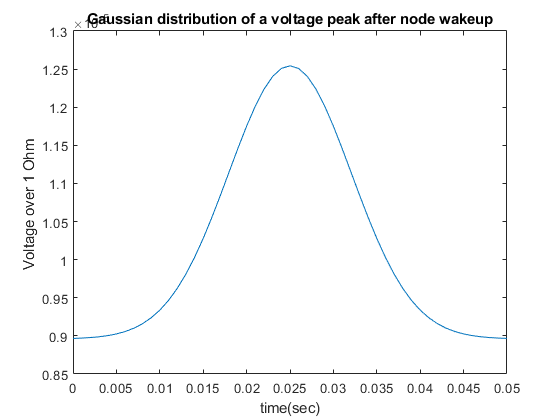
\includegraphics[width=\linewidth]{theory/energyCalculations/fig/gaussianDistributionsOfVoltagePeak.png}
	\caption{Start up voltage peak after sleep mode.}
	\label{fig:gaussianDistributionsOfVoltagePeak}
\end{figure}

\begin{table}[h]
	\centering
	\begin{tabularx}{\linewidth}{|l|r|l|X|r|}
		\hline
		\#	& Power		& Sleep	& Overshoot	& Lifetime	\\
		    & [dBm]		& 		& 		& [Hours]	\\ \hline
		1	& $0.0$		& No	& No	& 58.83		\\ \hline
		2	& $-25.0$	& No	& No	& 58.54		\\ \hline
		3	& $0.0$		& Yes	& No	& 4367.00	\\ \hline
		4	& $-25.0$	& Yes	& No	& 44396.00	\\ \hline
		5	& $0.0$		& Yes	& Yes	& 265.44	\\ \hline
		6	& $-25.0$	& Yes	& Yes	& 265.70	\\ \hline
	\end{tabularx}
	\caption{Half capacity battery lifetime table for the base station at different transmission powers and with/without sleep and overshoot.}
	\label{tab:halfLifetimeBaseStation}
\end{table}